\documentclass[11pt,a4paper,titlepage,oneside]{article}
\usepackage{LabProtocol}
\usepackage{tikz-timing}

\exercise{Exercise II}

% enter your data here
\authors{
	Cristian Avram, Matr. Nr. 01304470 \par
{\small e01304470@student.tuwien.ac.at} \par
}


\begin{document}

\maketitle

%%%%%%%%%%%%%%%%%%%%%%%%%%%%%%%%%%%%%%%%%%%%%%%%%%%%%%%%%%%%%%%%%%%%%%%%%%%%%%%%
%%%%%%%%%%%%%%%%%%%%%%%%%%%%%%%%%%%%%%%%%%%%%%%%%%%%%%%%%%%%%%%%%%%%%%%%%%%%%%%%
\Task{External Interface to AD7843}

Document the interface you designed for communication between the touch controller and the input manager.
Use Table \ref{tab:tc} for this purpose.

\begin{table}[h!]
	\centering
	\begin{tabular}{|l|l|l| p{0.8\textwidth}  |}
		\hline
		Signal & Mode & Width & Description \\\hline \hline
		x & out & 12 & This is the output(x-Coordinate) that $ Touch\_Controller $  gives, after it receives  as an input, the $ ADC\_DOUT $ Signal from ADConvertor\\ \hline
		y & out & 12 & This is the output(y-Coordinate) that $ Touch\_Controller $  gives, after it receives  as an input, the $ ADC \_ DOUT $ Signal from ADConvertor \\ \hline
		penirq$ \_ $n   & in & 1 &  Pen Interrupt Request. It's low active, when you touch the screen, it's 0\\ \hline
		busy & in & 1 & The 1 clock cycle between DIN and DOUT.\\ \hline
		dout & in & 1 &  The conversion resulted from the ADConvertor. It contains either X or Y Coordinate, depending on the DIN bits.\\ \hline
		scen & out & 1 & Is derived from SCEN Signal and when is 1, the ADConvertor is active. In the other case, the LCD and touch panel Module. Both can not be active at the same time. \\ \hline
		dclk & out & 1 & The clock used by the $ Touch\_Controller $ and ADConvertor.  \\ \hline
		din   & out & 1 & The 8bit ControlWord that is provided to the ADConvertor which contains information towards X or Y Coordinate. \\ \hline
	\end{tabular}
	\caption{Touch controller interface \label{tab:tc}}
\end{table}

Include a simulation screenshot (Figure \ref{fig:tc_timing_sim}) that shows how your touch controller forwards one coordinate pair of a single touch event (i.e.~x and y coordinate) to the input manager. 

%delete the figure that you don't use!

\begin{figure}[ht!]
	\centering
	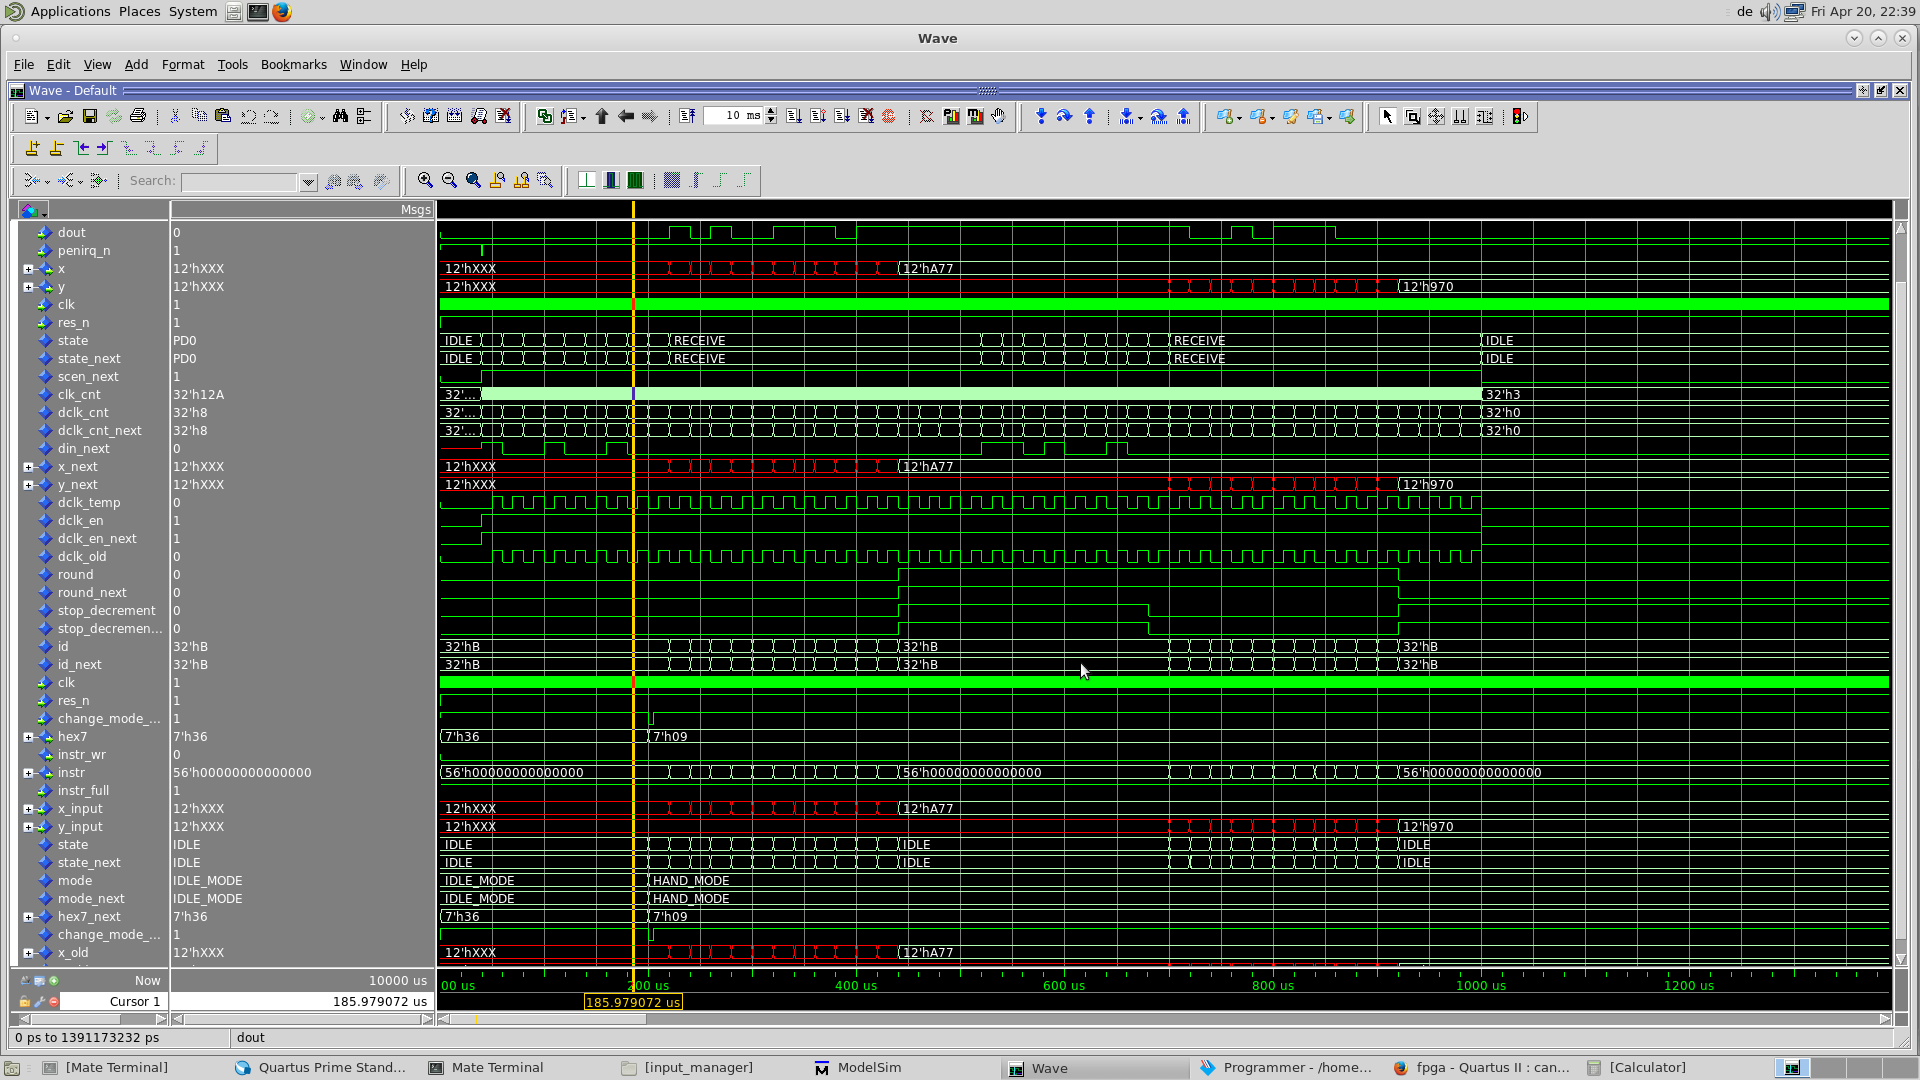
\includegraphics[width=1.0\linewidth]{Figure1.png}
	\caption{Simulation screenshot showing the touch controller interface \label{fig:tc_timing_sim}}
\end{figure}



\begin{qa}
	\question{What is the minimal time that must lie between the falling edge of the CS signal and the first rising clock edge of DCLK?}
	\answer{The minimum time that must lie between the falling edge of the CS signal and the first rising clock edge of DCLK is 10ns. This is the $ t_{1} $ from the ADConvertor Manual. }
\end{qa}

%%%%%%%%%%%%%%%%%%%%%%%%%%%%%%%%%%%%%%%%%%%%%%%%%%%%%%%%%%%%%%%%%%%%%%%%%%%%%%%%
%%%%%%%%%%%%%%%%%%%%%%%%%%%%%%%%%%%%%%%%%%%%%%%%%%%%%%%%%%%%%%%%%%%%%%%%%%%%%%%%
\Task{Internal interface to the graphics controller}

\begin{figure}[ht!]
	\centering
	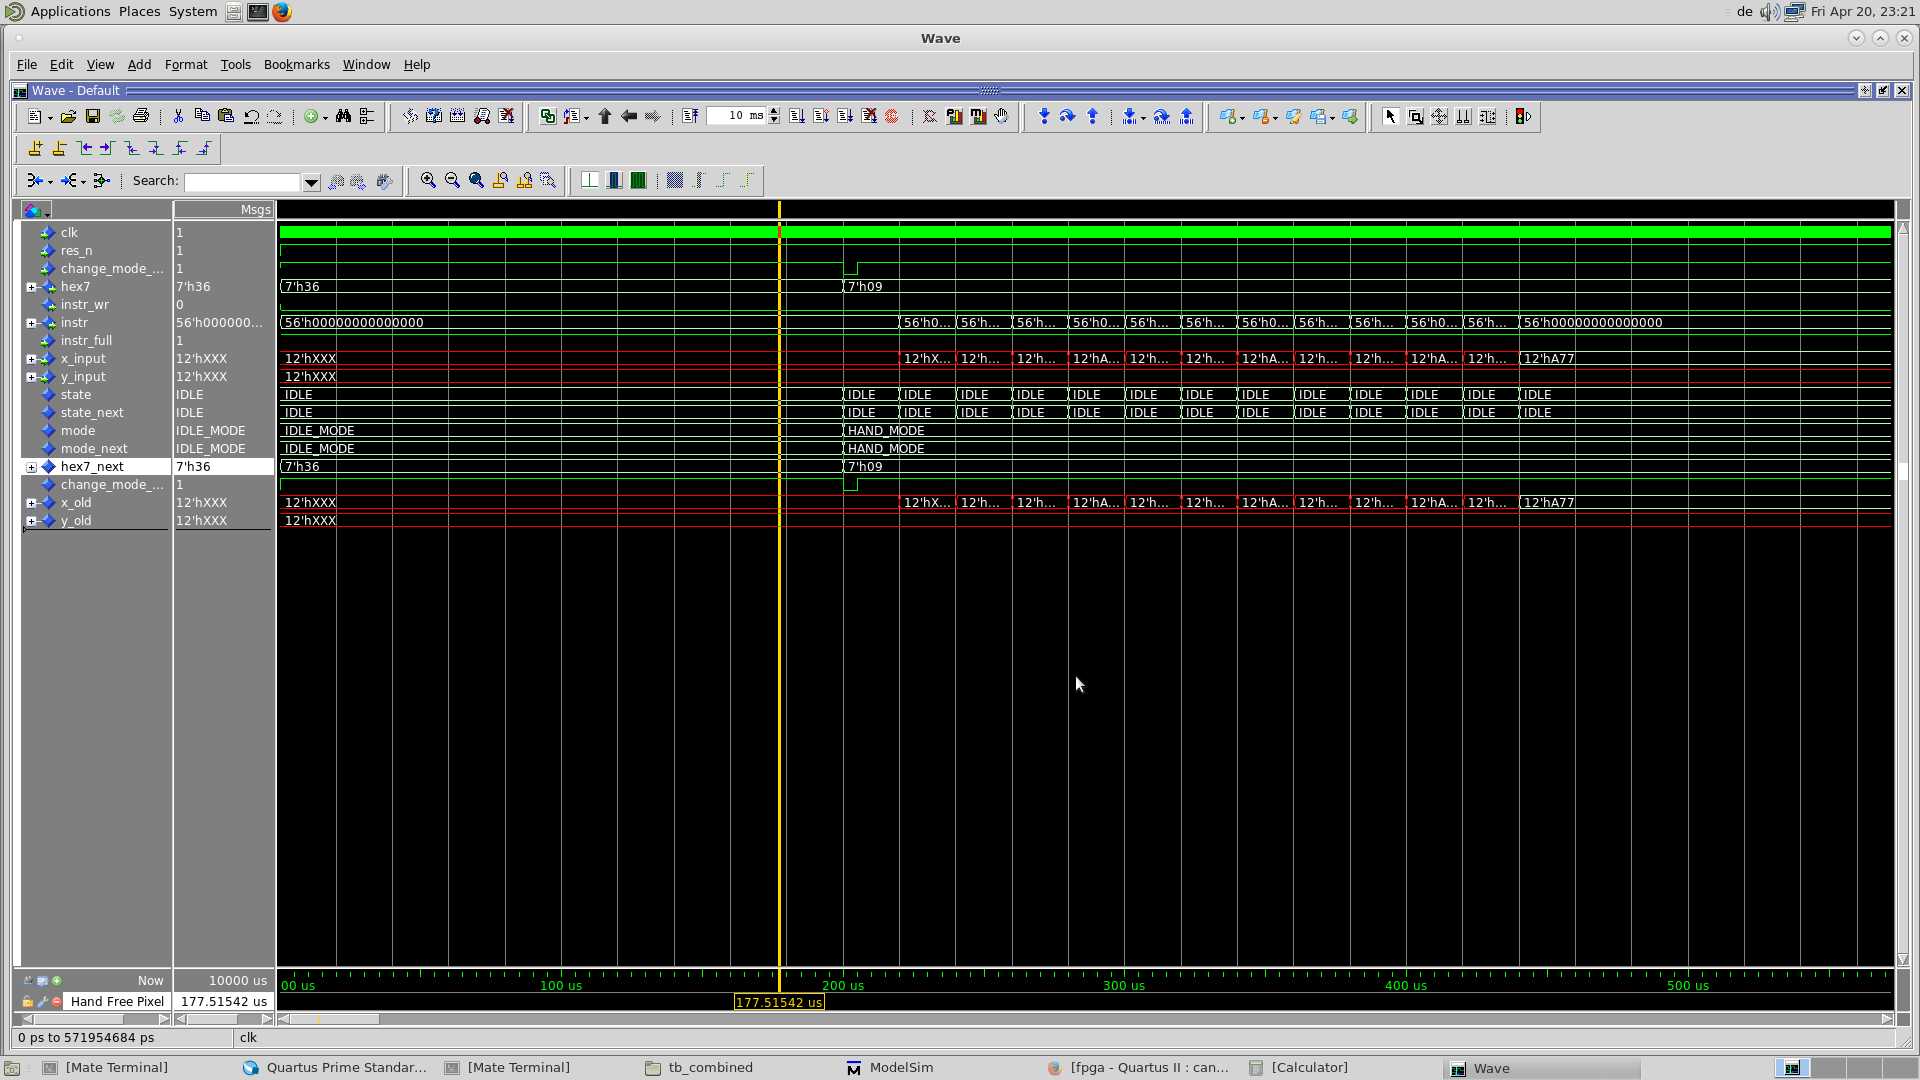
\includegraphics[width=1.0\linewidth]{Figure2.png}
	\caption{Simulation screenshot demonstrating the Free-Hand mode}
\end{figure}

%%%%%%%%%%%%%%%%%%%%%%%%%%%%%%%%%%%%%%%%%%%%%%%%%%%%%%%%%%%%%%%%%%%%%%%%%%%%%%%%
%%%%%%%%%%%%%%%%%%%%%%%%%%%%%%%%%%%%%%%%%%%%%%%%%%%%%%%%%%%%%%%%%%%%%%%%%%%%%%%%
\Task{Integration}

\begin{table}[h!]
	\centering
	\begin{tabular}{|l|l|l|l|}
	\hline
	& LC Combinationals & LC Registers & Memory      \\ \hline 
	Absolute number      &        324           &     152         &      0       \\ \hline
	\end{tabular}
	\caption{Combined resource usage of the touch controller and input manager }
\end{table}

%%%%%%%%%%%%%%%%%%%%%%%%%%%%%%%%%%%%%%%%%%%%%%%%%%%%%%%%%%%%%%%%%%%%%%%%%%%%%%%%
%%%%%%%%%%%%%%%%%%%%%%%%%%%%%%%%%%%%%%%%%%%%%%%%%%%%%%%%%%%%%%%%%%%%%%%%%%%%%%%%



\end{document}
